\documentclass[tikz,border=4pt]{standalone}
\usetikzlibrary{shapes.geometric, arrows, positioning}
\begin{document}
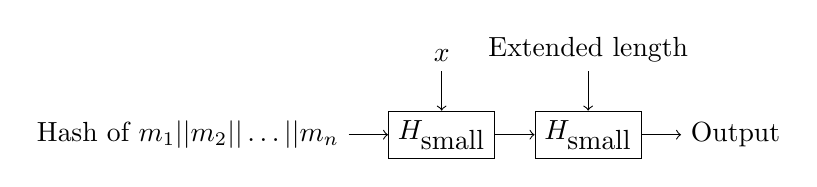
\begin{tikzpicture}
    \node (start) {Hash of $m_1 || m_2 || \ldots || m_n$};
    \node [right=.5cm of start] (H1) [draw] {$H_\textrm{small}$};
    \draw [->] (start) edge (H1);
    \node [above=.5cm of H1] (x) {$x$};
    \draw [->] (x) edge (H1);
    \node [right=.5cm of H1] (Hfinal) [draw] {$H_\textrm{small}$};
    \draw [->] (H1) edge (Hfinal);
    \node [above=.5cm of Hfinal] (len) {Extended length};
    \draw [->] (len) edge (Hfinal);
    \node [right=.5cm of Hfinal] (out) {Output};
    \draw [->] (Hfinal) edge (out);
\end{tikzpicture}
\end{document}
